
\chapter{协议实现}

第一周的协议实现主要分为“消息解析”和“消息反馈” 两个部分。

\section{消息解析}

\begin{figure}[htbp!]
    \centering
    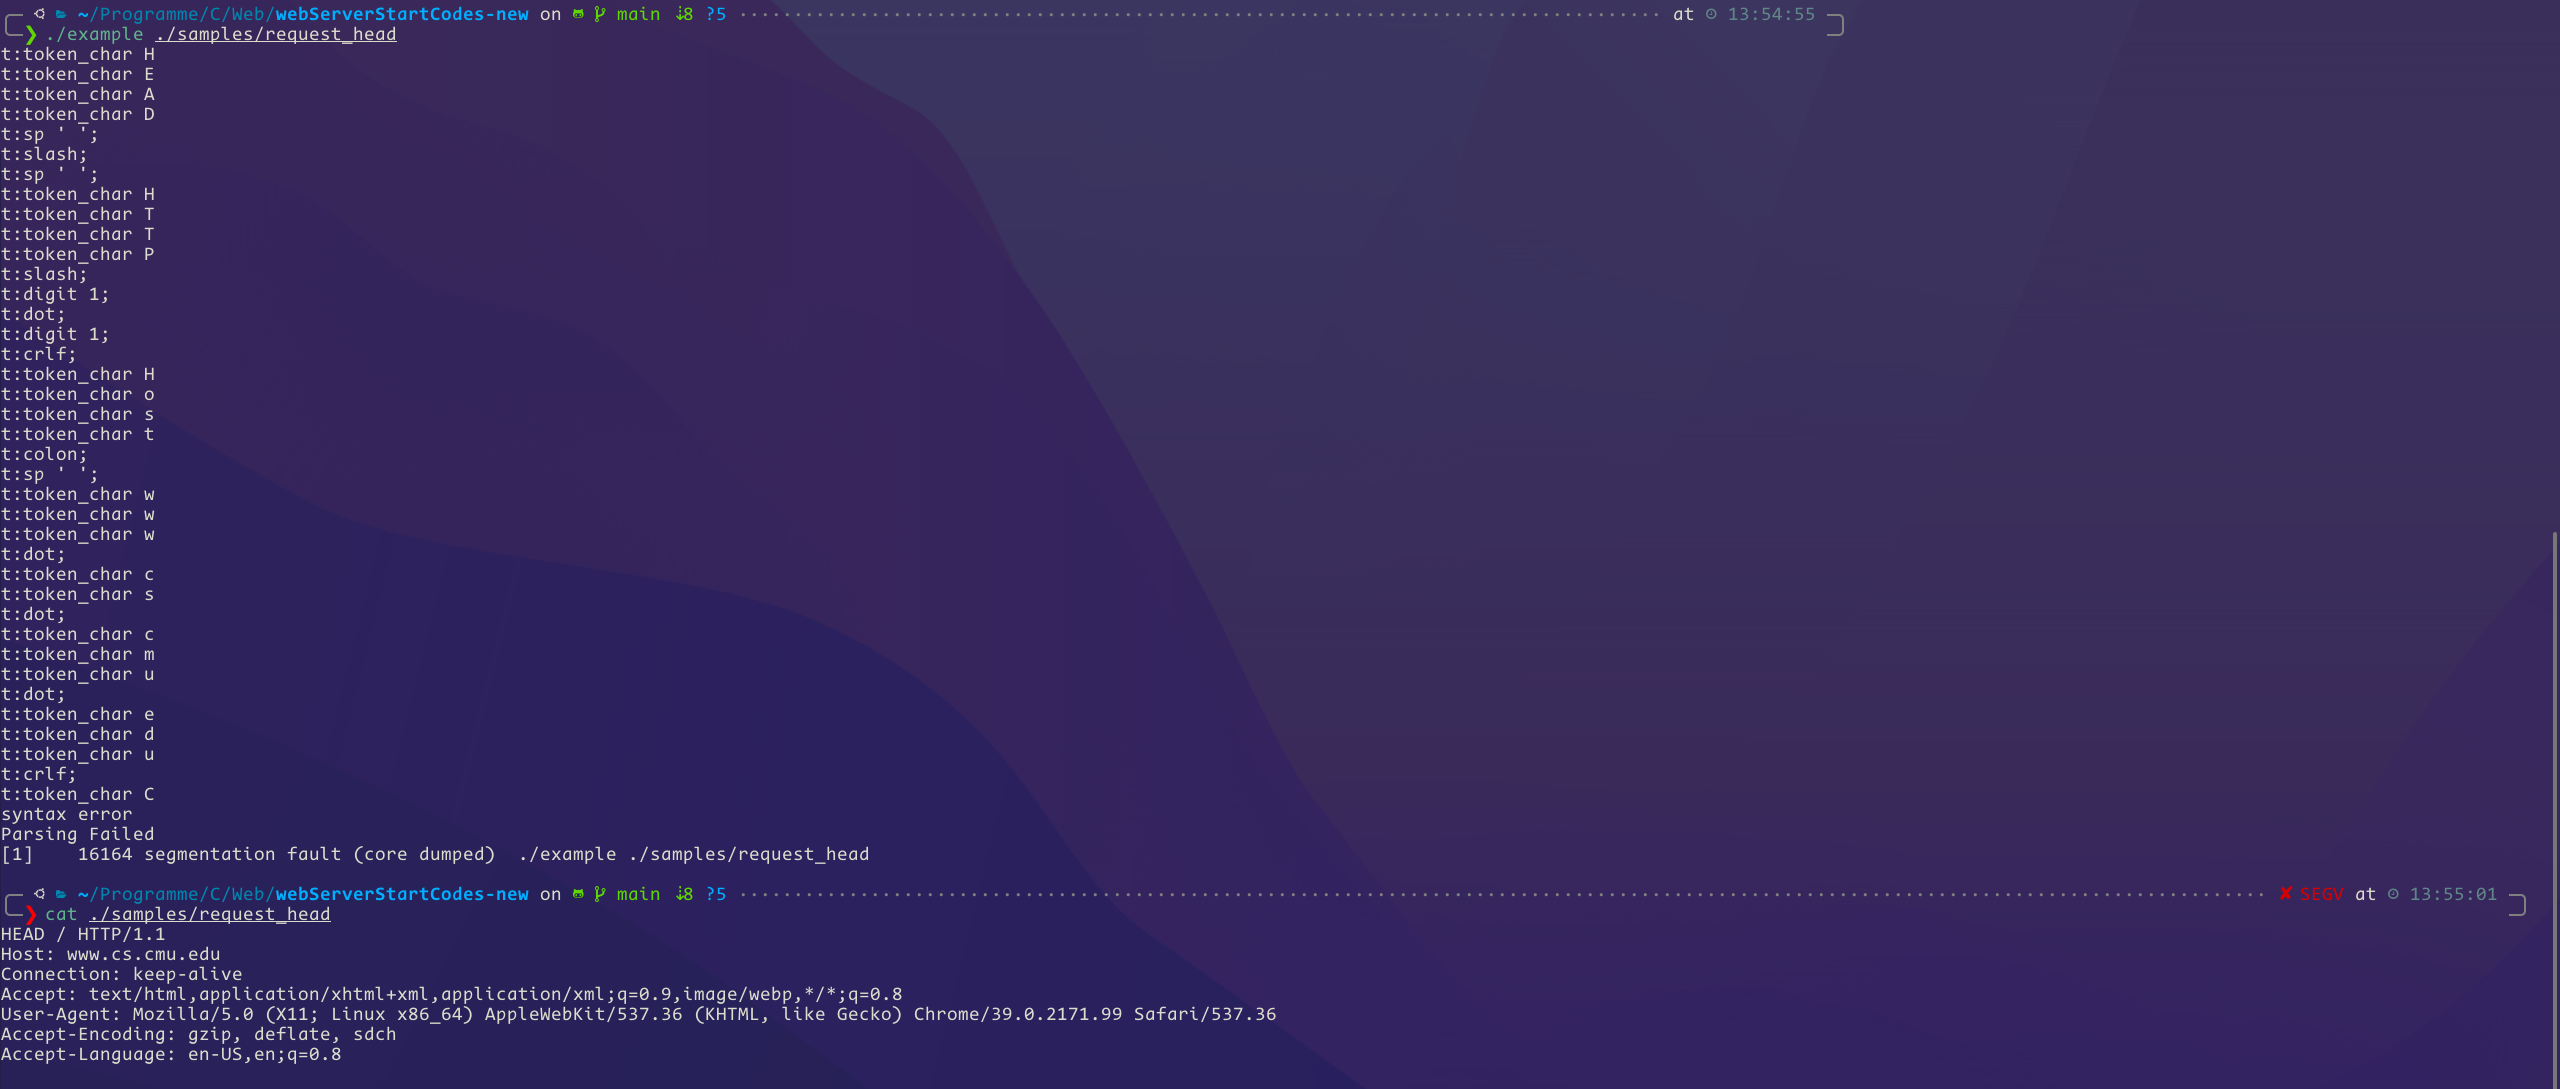
\includegraphics[width=4.5in]{segmentFault.png}
    \caption{Segment Fault}\label{fig:segmentfault}
    \vspace{-1em}
\end{figure}

如图\ref{fig:segmentfault},通过 example.c 的测试,我们发现了第一个错误: Segment fault,且该错误总是在解析第三行消息时出现。

通过对 parser.y 和 parse.h 文件的理解,我们认为此问题应该出自其 Request 中 Request\_header,它在最初定义时是一个指针 *header,所以在解析第二行时没有错误,而在进行第三行即以后的解释时,如果不进行人为的空间分配,则当然会出现上述的 Segment Fault。

所以对于这个问题,我们只需在 parser.y 中进行修改,增加 realloc 的函数,对 header 进行扩容,并且相应的 grammar 与之对应即可。

当然,还可以在 example.c 中处理一下返回错误的情况,避免直接访问 NULL 的空间导致 Segment Fault。使用批量脚本测试则效果如图\ref{fig:maketestexample}。

\begin{figure}[htbp!]
    \centering
    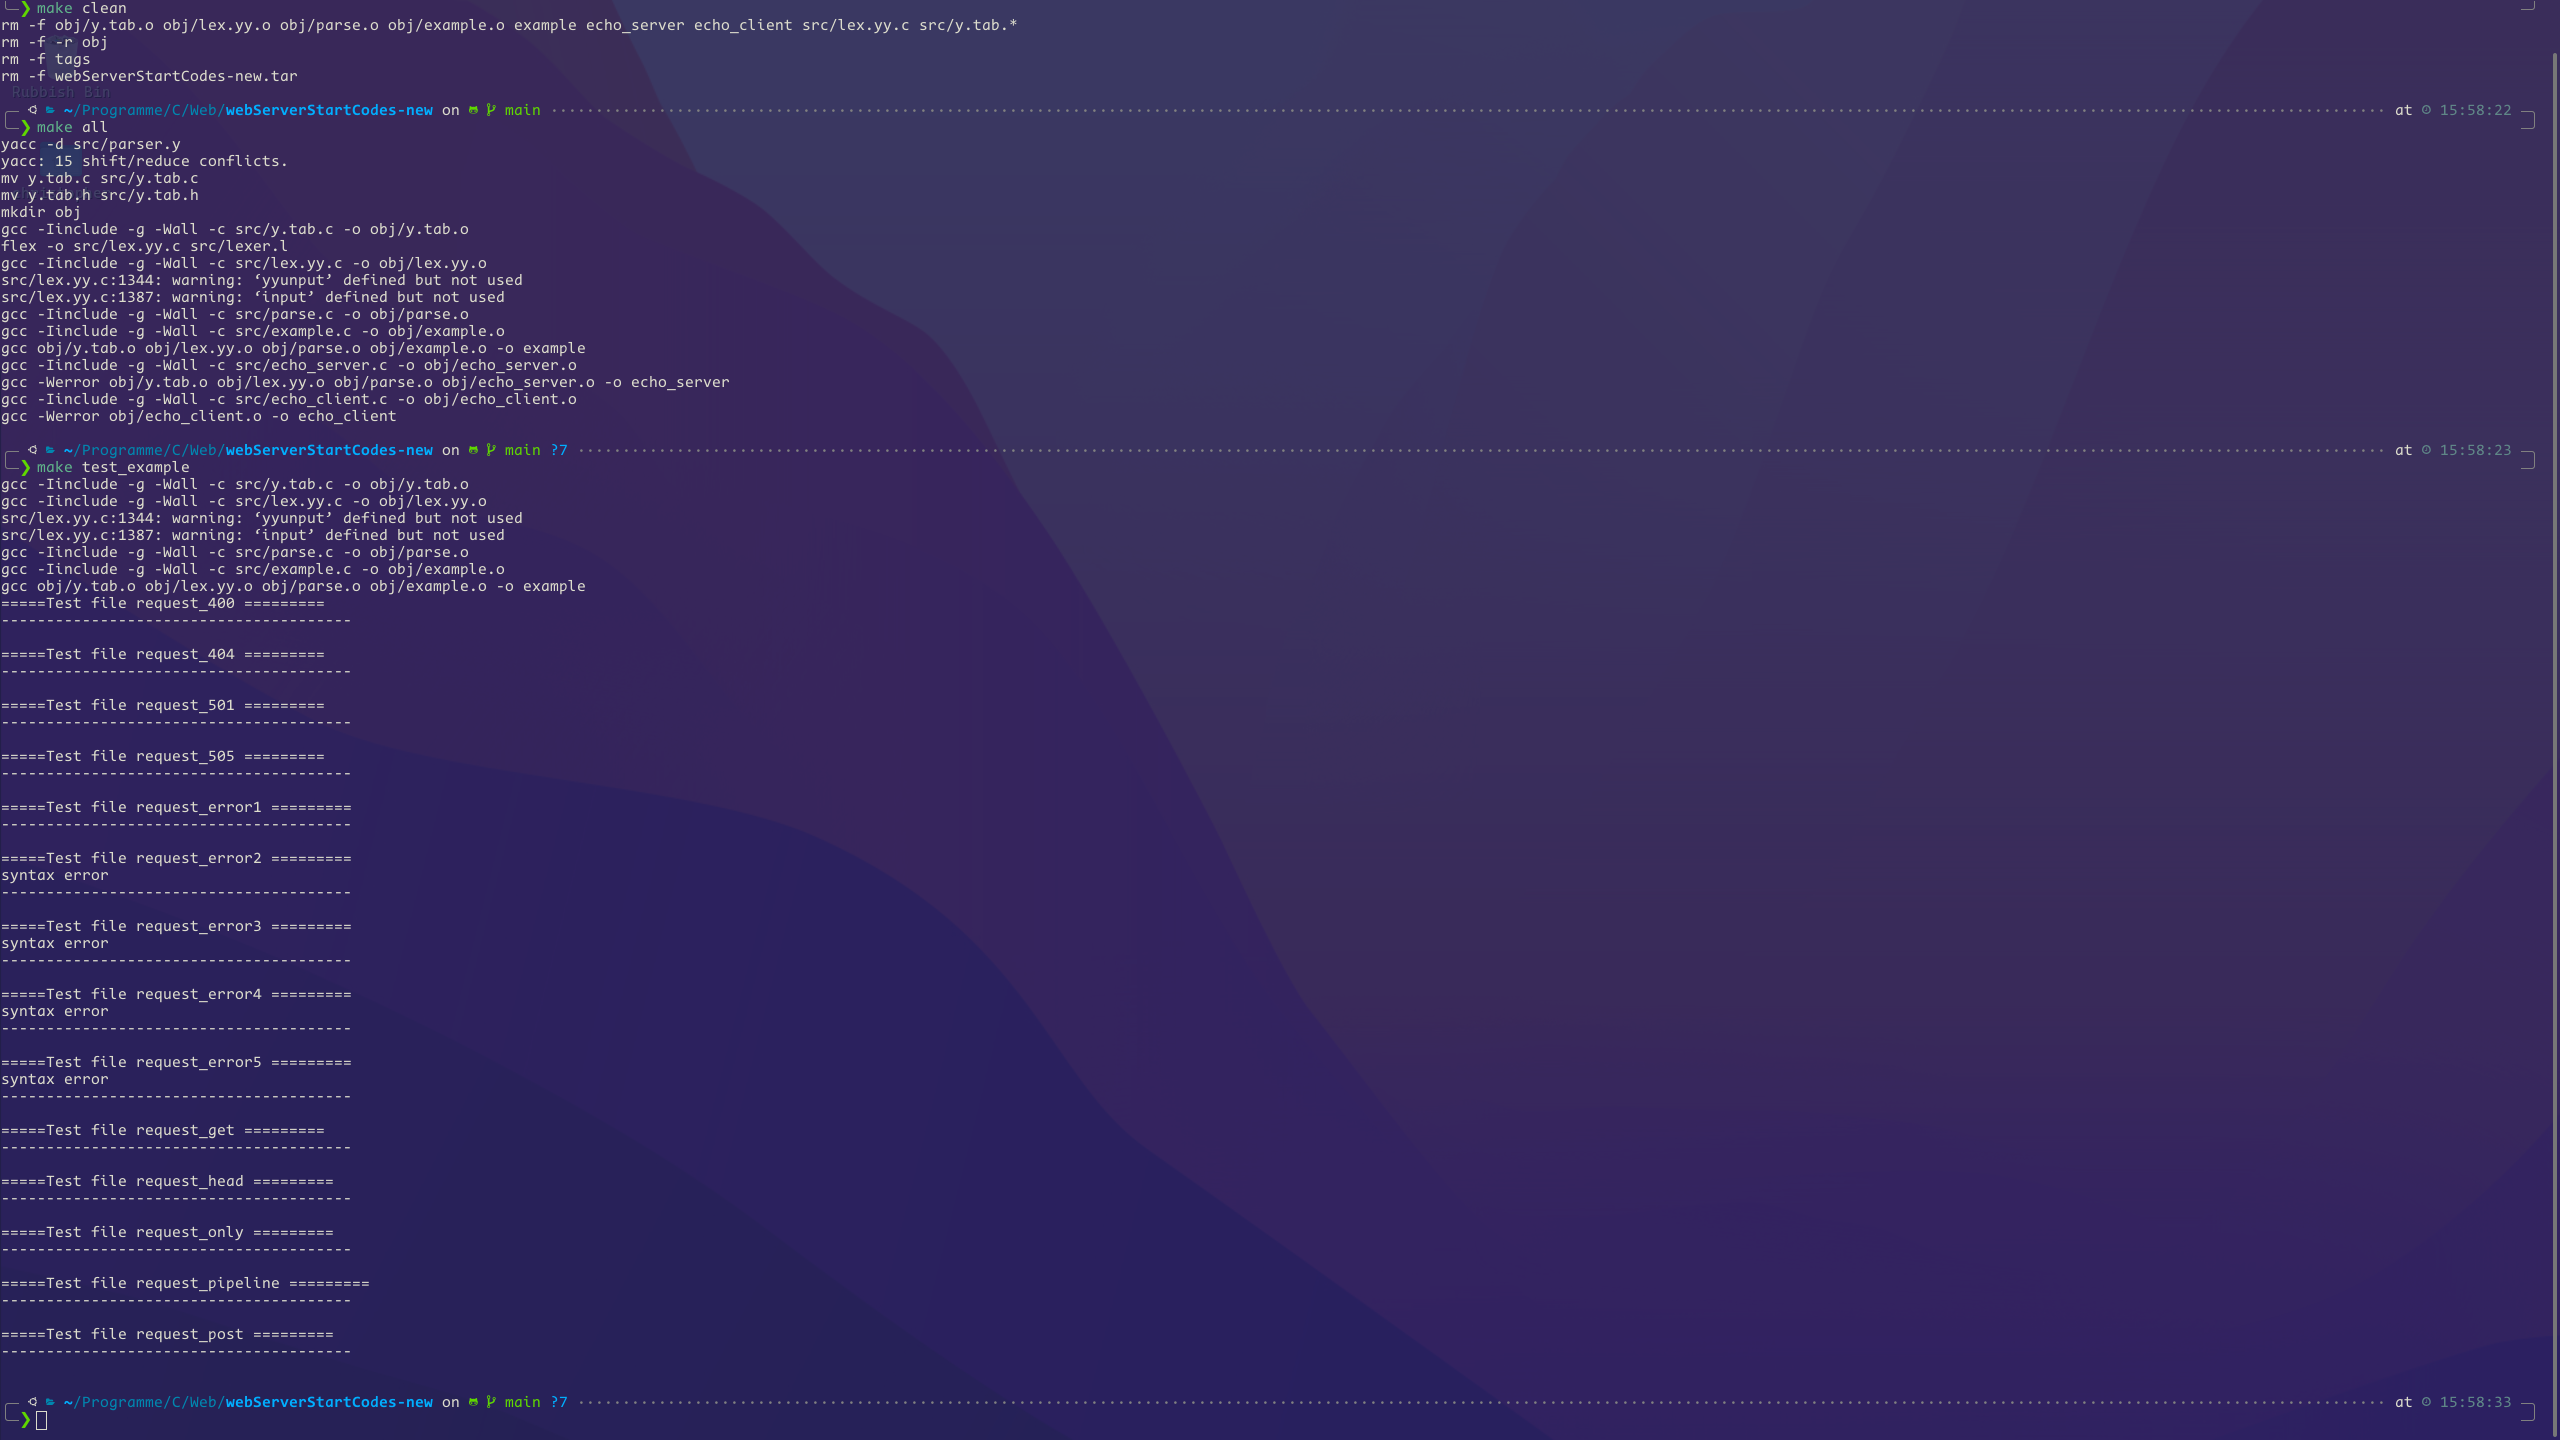
\includegraphics[width=4.5in]{make_test_example.png}
    \caption{Example Test}\label{fig:maketestexample}
    \vspace{-1em}
\end{figure}

\section{消息反馈}

在完成消息解析后,我们对 echo\_server.c 进行编程,完成消息的解析、处理与返回。研读源代码,梳理出如 "echo\_server" 代码段的伪代码。

我们只需要在第 7 行 "TODO: DEAL WITH MESSAGE" 处增加如代码段 “处理数据” 的 “解析、分类、封装返回值” 即可。

\begin{itemize}
    \item 具体而言,先通过 example.c 一样的方法解析 buf 中收到的数据。在该步骤中,可能会出现依赖问题,对此我们需要在 Makefile 中增加相关的依赖。让 echo\_server 在连接时加上 parse.o 的文件即可。
    \item 得到 request 后,我们对 request 的两种情况进行分析
    \item 如果 request 为 NULL,则解析不成功,即返回 400 错误
    \item 如果 reqeust 成功,但是发现其中 method 暂不支持,则返回 500 错误
    \item 否则直接返回受到的数据
\end{itemize}

\begin{lstlisting}[language=python, name={echo_server}]
create socket
bind socket
listen on socket
while(1):
    accept connection
    while(recieve message):
        TODO: DEAL WITH MESSAGE
        send back
    close client socket
close socket
\end{lstlisting}
    
\begin{lstlisting}[language=python, name={处理数据}]
def deal_with_request(buf):
    Request *request = parse(buf, BUF_SIZE, 8192)
    if request is NULL:
        return _400msg
    if method_not_support:
        return _500msg
    return buf
\end{lstlisting}


